\documentclass[12pt,letterpaper]{article} 
\usepackage[letterpaper,margin=1in]{geometry} 
\usepackage{mathptmx}
\usepackage[singlespacing]{setspace}
\usepackage{fancyhdr}
\setlength{\headheight}{14.49998pt}
\usepackage{relsize}
\usepackage[bottom]{footmisc}
\usepackage{tabularx}
\setlength{\parindent}{2em}
\usepackage{url}
\usepackage{hyperref}
\usepackage[english]{babel}
\usepackage{graphicx}
\usepackage{booktabs}
\usepackage{natbib}
\usepackage{expex}
\usepackage{amsfonts} 
\usepackage{tikz}
\bibpunct[:]{(}{)}{;}{a}{}{,}
\usepackage{bibentry}
\usepackage{acronym}
\usepackage{multicol}
\author{Ruben Triwari}
\usepackage{scrhack} 
\usepackage{microtype}
\usepackage[acronym,xindy,toc]{glossaries}
\makeglossaries
\loadglsentries{glossary.tex}
\usepackage{ragged2e}
\babelhyphenation[english]{
an-oth-er
ex-am-ple
}
\newtheorem{definition}{Definition}
\newtheorem{example}{Example}[section]
\newenvironment{proof}{\paragraph{Proof:}}{\hfill$\square$}
\usepackage{dcolumn}
\newcolumntype{2}{D{.}{}{2.0}}
\usetikzlibrary{
  automata, positioning,
  arrows, matrix, decorations.pathreplacing,
  shapes.geometric
}
\newcommand{\fps}[1] {
\mathbb{#1}\langle \langle \Sigma^* \rangle \rangle
}

\tikzset{ 
  table/.style={
    matrix of math nodes,
    row sep=-\pgflinewidth,
    column sep=-\pgflinewidth,
    nodes={rectangle,text width=3em,align=center},
    text depth=1.25ex,
    text height=2.5ex,
    nodes in empty cells,
    left delimiter=[,
    right delimiter={]},
    ampersand replacement=\&
  }
}

\begin{document}

\begin{center}\uppercase{Ludwig-Maximilians-Universität München}\end{center}
\begin{center}\uppercase{Chair of Theoretical Computer Science and Theorem Proving}\end{center}

\vspace*{10mm}
\begin{center}
\includegraphics[height=40mm]{sigillum.png}
\end{center}
\vspace*{10mm}
\title{Formal Languages and Automatas}
\date{\vspace{-3ex}}
{\let\newpage\relax\maketitle}
\thispagestyle{empty}

\begin{center}
\begin{large}
\begin{Large}
Seminar Paper on Formal Languages and Automata\\
\end{Large}
for the course ``Algebra \& Computer Science'' \\
\end{large}
\end{center}
\vspace{1cm}
\begin{center}
\begin{large}
Supervisor: Prof. Dr. Jasmin Blanchette\\
\end{large}
\end{center}
\begin{center}
\begin{large}
Advisor: Xavier Genereux\\
\end{large}
\end{center}


\begin{center}
\begin{large}
Submission Date: \date{\today} \\
\end{large}
\end{center}

\vspace{1,5cm}
\cleardoublepage{}
\thispagestyle{empty}
\vspace*{0.8\textheight}
\noindent
\makeatletter
\begin{center}
{\normalfont\bfseries} Disclaimer
\end{center}
\begin{flushleft}
I confirm that this seminar paper is my own work and I have documented all sources and material used.\\
\makeatother
\vspace{15mm}
\noindent
Munich, \date{\today} \hspace{50mm} Author
\end{flushleft}
\cleardoublepage{}

\newpage
\tableofcontents
\newpage

\setcounter{page}{1}
\pagestyle{fancy}
\fancyhf{}
\fancyhead[R]{\thepage}
\renewcommand{\headrulewidth}{0pt} %obere Trennlinie

\section{Introduction}
This paper aims to give a gentle introduction to the world of
automata with formal power series. Formal power series are really
useful for weighted automata, but not so much for the topics we are
covering in this paper. Thus, some proofs may not be as simple as in 
other literature. First, we will go over some definitions, starting
from scratch, but ending up with the definition of an automaton using
a matrix and  formal power series. In the third chapter, we will
provide some intuition as to why one would use a formal power
series in this context and show that the definition of formal 
language using formal power series and sets is equivalent.
At the end of the third chapter, we will discuss why formal power 
series are so powerful in the context of automata theory.
In the fourth chapter, we will prove the kleene's theorem using the
formal power series representation of sets. 
At the end, we will give  an outlook on weighted automata.

\section{Backround}
Firstly, we need to define some structures and ideas, 
that will be really important in this paper.
We will define  formal languages in two ways and then 
the automata accordingly. 
A formal language is just a set of words, where words are
a series of characters from an alphabet
\begin{definition}
  An Alphabet is an abritrary non empty finite set denoted with $\Sigma$
\end{definition}
\begin{example} Simple examples for Alphabets would be:
  \begin{enumerate}
    \item $\Sigma = \{x\}$
    \item $\Sigma = \{a,b,c,d, \dots z \}$
    \item $\Sigma = \{1,2,3, \dots n \}$ where $n \in \mathbb{N}$
  \end{enumerate}
\end{example}
This definition is rather general, because an alphabet $\Sigma$
can really be anything. We could also define an alphabet as a subset of
the natural numbers $\Sigma \subset \mathbb{N}$. This is equivalent to
the previous definition, because we can always find a one-to-one map between
a finite amount of objects and the natural numbers. In other words 
we can always enumerate a finite amount of objects. The above definition
results in more readable words, thus resulting in more readable problems.
Furthermore, it's unintuitive to have words full of numbers and languages full of number series. That is why we are choosing this definition, like most
of the literature.\\
Now that our first building block is defined, we can define words, which are just
a series of characters in an alphabet.
\begin{definition}
  Let $\Sigma$ be an fixed alphabet, then $w$ is a series of characters out of
  $\Sigma$. 
  \[
    w = (a_1,a_2, \dots, a_n) \in \Sigma^n
  \]
  We will denote it by:
  \[
    w = a_1a_2\dots a_n
  \]
  The empty word which contains no characters, 
  and is denoted by $\epsilon$.
  %book schützenbert
\end{definition}
\begin{example}
  Simple examples for words would be:
  \begin{enumerate}
    \item $\Sigma = \{a,b,c\} \rightsquigarrow w_1 = abc$
    \item $\Sigma = \{x\} \rightsquigarrow w_2 = xxxx$
    \item $\Sigma = \{1,2,3\} \rightsquigarrow w_3 = 112233$
    \item $\Sigma = \{1,2,3\} \rightsquigarrow w_4 = \epsilon$
  \end{enumerate}
\end{example}
The empty word $\epsilon$ is analogous to the empty set in set theory.
It has a lot of uses, but one obvious one is that now one can define 
a monoid over words $(M, \cdot, \Sigma, \epsilon)$.
M is a set of words and multiplication is the concatenation of words, then 
$\epsilon$ is the neutral element of the monoid. Which brings us to
the next definition.
\begin{definition}
  Let $\Sigma$ be an fixed alphabet and  $w$, $v$ words with 
  characters out of $\Sigma$. Then the contenation is defined by:
  \[ w \cdot v := wv\]
  sometimes just written as $wv$. With powers recursively defined by:
  \begin{align*}
    w^0 &:= \epsilon\\
    w^1 &:= w\\
    w^{n+1} &:= w^n\cdot w
  \end{align*}
\end{definition}
In simple terms, a concatenation of two words is just a new word with
the two words were chained together. Now we can again build on
words to define languages.
\begin{definition}
  Let $\Sigma$ be an fixed alphabet, then a formal language is a 
  set of words, with characters in $\Sigma$.
\end{definition}
\begin{example}
  Simple examples for formal languages would be:
  \begin{enumerate}
    \item $\Sigma = \{a,b,c\} \rightsquigarrow L = \{aaa, bbb, ccc, abc\}$
    \item $\Sigma = \{x\} \rightsquigarrow L = \{ x, xx, xxx, xxxx\}$
    \item $\Sigma = \{1,2,3\} \rightsquigarrow L = \{11, 22, 33, 123,\epsilon\}$
  \end{enumerate}
\end{example}
This definition is really clear and simple. We will see a less intuitive way to
define language shortly. Obviously, the simpler one has some downsides, 
which we will discuss later in the paper. \\
The kleene star $^*$ is a really powerful operator, to define it, we need
to first define contention for languages.
\pagebreak
\begin{definition}
  Let $\Sigma$ be an fixed alphabet and  $L$, $V$ languages with 
  words constructed out of $\Sigma$.
  Then the contenation of formal languages is defined by:
  \[ L \cdot V := \{ l \cdot v | l \in L \land v \in V \}\]
  sometimes just written as $LV$. With powers defined recursively:
  \begin{align*}
      L^0 & := \{\epsilon \}\\
      L^1 & := L  \\
      L^{i+1} & := \{ l_i\cdot l | l_i \in L^i \land l \in L\}
  \end{align*}
  % wikipedia kleene star
\end{definition}
In simple terms, we are creating a new language by
combining every word of the first language with every word of
the second. Now we are able to define the kleene star operator
\begin{definition}
  Let $\Sigma$ be an fixed alphabet and  $L$  a language with 
  words constructed out of $\Sigma$.
  Then the kleene star of  a formal language is defined by:
  \[ 
    L^* := \bigcup_{i \in \mathbb{N}_0} L^i = 
    L^0 \cup L^1 \cup L^2 \cup \dots
  \]
  and 
  \[ 
    L\hat{\mkern6mu} := \bigcup_{i \in \mathbb{N}} L^i = 
     L^1 \cup L^2 \cup L^3 \cup \dots
  \]
\end{definition}
In simple terms, it generates all possible permutations of arbitrary length of a formal language. This is really powerful, because $\Sigma^*$ is the
biggest language one can construct from the alphabet $\Sigma$. Thus, every  language $L$ generated by $\Sigma$ is just a subset of $\Sigma^*$.\\
Unintuitively, we can also write a formal language as a formal power series.
\begin{definition}
  Let $\Sigma$ be an fixed alphabet, then a formal language can be 
  written as formal power series $L$:
  \[
    L: \Sigma^* \to \mathbb{B}
  \]
  where
  \[
    \mathbb{B} = \{0, 1\}
  \]
  \[
    L = \sum_{w \in \Sigma^*} (L,w)w \verb| where | 
    (L,w) \in \mathbb{B}.
  \]
  {\bf Note:} The set of formal power series is denoted by 
  $\mathbb{B}\langle \langle \Sigma^* \rangle \rangle 
    = \{ \Sigma^* \to \mathbb{B}\}$\\
  {\bf Notation:} If the language consist only out of one 
  character or the empty word $a \in \Sigma \cup \{\epsilon\}$, 
  then the formal power series would be: 
  \[
    L = h \in \fps{B}
  \]
  where 
  \[
    h: \Sigma^* \to \mathbb{B}
  \]
  \[
    h(w) = 
    \begin{cases}
      1 & \text{if   } w=a \\
      0 & \text{otherwise}
    \end{cases}.
  \]
  In this case we just write $L = a$.
  The language with no words is denoted by $L = 0$.
    %schützenberg
\end{definition}
This looks like a sum, we call it a series, but it is actually a map from 
words to zero or one. The sum is a way to write a function definition: In front of every word $w \in \Sigma^*$ in the series, there is a $x \in \mathbb {B}$, which is zero or one. So we can interpret every element in the series as an 
assignment: $w \mapsto x$.
All words that map to one are in the language, the others are not. So we can write a formal language as a function $\Sigma^* \to \mathbb{B}$.\\
The representation with sets has the advantage that a formal language
will inherit all operations on sets like complement, union, and intersection.
Those operations are really useful, so we will define similar ones on the power
series version.
\begin{definition}
  Let $\Sigma$ be an fixed alphabet and $L, V \in \mathbb{B}\langle \langle
  \Sigma^* \rangle \rangle$, where
  \[
    L = \sum_{w \in \Sigma^*} (L,w)w \hspace{0.5cm} \text{and} \hspace{0.5cm}
    V = \sum_{w \in \Sigma^*} (V,w)w.
  \]
  Addition and multiplication on formal power series is defined
  as follows:\\
  \[
    L + V := \sum_{w \in \Sigma^*} ((L,w) + (V,w))w
    \hspace{0.5cm} \text{and} \hspace{0.5cm} 
    L \cdot V := \sum_{\substack{u,v \in \Sigma^* \\ w = uv }} 
      ((L,u) \cdot (V,v))w
  \]
  This definition is not recursive, because the right addition and 
  muliplication operater are from the Boolean Algebra 
  $\mathbb{B} = \{0,1\}$.
  \begin{center}
    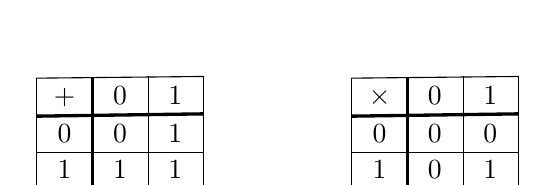
\begin{tikzpicture}
      \matrix (m) [nodes={minimum width=2em,minimum height=2ex},matrix of nodes]
      {
      $+$&0&1\\
      0&0&1\\
      1&1&1\\
      };
      \draw[very thick] (m-1-1.north east) -- (m-3-1.south east);
      \draw[very thick] (m-1-1.south west) -- (m-1-3.south east);
      \draw (m-1-1.north west) -- (m-3-1.south west);
      \draw (m-1-1.north west) -- (m-1-3.north east);
      \foreach \x in {2,...,3}{
        \draw (m-1-\x.north east) -- (m-3-\x.south east);
        \draw (m-\x-1.south west) -- (m-\x-3.south east);
      }

      \matrix [
        nodes={minimum width=2em,minimum height=2ex}
        ,matrix of nodes
      ] at (4,0)
      {
        \node(a){$\times$}; & \node(b){0}; & \node(c){1}; \\
        \node(d){0}; & \node(e){0}; & \node(f){0}; \\
        \node(g){1}; & \node(h){0}; & \node(i){1};\\
      };
      \draw[very thick] (a.south west) -- (c.south east);
      \draw[very thick] (a.north east) -- (g.south east);

      \draw (a.north west) -- (c.north east);
      \draw (a.north west) -- (g.south west);

      \draw (b.north east) -- (h.south east);
      \draw (d.south west) -- (f.south east);

      \draw (c.north east) -- (i.south east);
      \draw (g.south west) -- (i.south east);

    \end{tikzpicture}
  \end{center}
  With powers defined recursively:
  \begin{align*}
    L^0 &:= \epsilon\\
    L^1 &:= L\\
    L^{i+1} &:= \sum_{\substack{u,v \in \Sigma^* \\ w = uv}}
    ((L^i,u)\cdot (L,v))w, 
  \end{align*}
  Kleene Star can now also be defined for formal power series:
  \[
    L^* := L^0 + L^1 + L^2 + L^3 + \dots = \sum_{i \in \mathbb{N}_0} L^i.
  \]
  and
  \[
    L\hat{\mkern6mu} :=  L^1 + L^2 + L^3 + \dots = \sum_{i \in \mathbb{N}_0} L^i.
  \]
\end{definition}
With these operation defined our two versions of formal languages are 
powerful tools, which will be compared in the following sections. In order
to conpare them we will also need finite automatas. Simillar to formal languages
there are multiple ways one can define finite automatas. In this paper we
will define two. One is more suitable for combining it with the set version
of formal languages and the other one is more siutable for the formal power
series representation. First we will define the one more suitable for the
set version.
\begin{definition}
  A finite automata is a quintuple $M = (Q, \Sigma, \delta, q_0, F)$, 
  where
  \begin{enumerate}
    \item Q is a finite set of states,
    \item $\Sigma$ is an alphabet, all inputs are constructed from,
    \item $\delta: Q \times \Sigma \to Q$ is the transition function,
      carrying the automata from one state to another,
    \item $q_0 \in Q$ is the initial state of the automata,
    \item $F \subset Q$ are the accepting states of the automata.
  \end{enumerate}
  %Definition is out of theoretical computer science book (german)
\end{definition}
In simple terms, a finite automaton gets an input string and a starting  state. Then it works through the input string, starting at the first character and carrying the starting state to another according to the transition function.
Exactly the same procedure applies for the second input string character and the remaining characters. If this process ends up in an accepting state, the automata accept the input string. Consequently, the finite automata generate a language, namely the words that the automata 
accepts. The definition above is one possible way to encode a finite automaton. 
Like with graphs, we can encode the transition function of a finite
automata, with just a matrix.
\begin{definition}
  Let $M = (Q, \Sigma, \delta, q_0, F)$ be an abitrary finite 
  automata, where $Q = \{ s_1, s_2, \dots s_n\}.$ \\
  Frthermore, we need a helper function:
  \[
    \delta': \mathbb{N} \times \mathbb{N} \to \fps{B}
  \]
  where
  \[
    \delta'(i, j) = 
      \begin{cases}
        \alpha, & \text{if} \hspace{0.2cm} \exists \alpha \in \Sigma: 
          \delta(s_i, \alpha) = s_j \\
        0, & \text{otherwise}
      \end{cases}.
  \]
  Then the finite automata $M$ can be encoded with a Matrix
  $A \in \fps{B}^{n \times n}$
  in the following way:
  \[
    A = 
    \begin{pmatrix}
      \delta'(1,1)       & \delta'(1,2) & \delta'(1,3) & \dots & \delta'(1,n) \\
      \delta'(2,1)       & \delta'(2,2) & \delta'(2,3) & \dots & \delta'(2,n) \\
      \vdots             & \vdots       & \vdots       & \ddots& \vdots\\
      \delta'(n,1)       & \delta'(n,2) & \delta'(n,3) & \dots & \delta'(n,n) \\
    \end{pmatrix}
  .\]
  We can denote a state transition $s_i \to s_j$ with $s_iA_{ij} = s_j$.\\
  {\bf Note:} We definined $A \in \fps{B}^{n \times n}$ and not 
  $A \in \Sigma^{n \times n}$, because otherwise the defintion is not closed
  under matrix multiplication, nor matrix addition.
  \pagebreak\\
  The kleene star of a Matrix can intuively be defined as:
  \[
    A^* = E_n + A + A^2 + A^3 \dots  = \sum_{i \in \mathbb{N}_0} A^i
  \]
  and
  \[
    A\hat{\mkern6mu} = A + A^2 + A^3 \dots  = \sum_{i \in \mathbb{N}} A^i
  \]
  where
  \[ E_n \in \fps{B}^{n \times n}\]
  \[
    (E_n)_{ij} := 
    \begin{cases}
      \epsilon & \text{if } \hspace{0.2cm} i=j \\
      0        & \text{otherwise}
    \end{cases} \in \fps{B}
  \]
  Now, we can write our finite automata in a shorter way:
  \[
    M' = (\Sigma, A, q_0, F)
  \]
\end{definition}
This definition only works, because we have finite sets. Note that we can omit
the state set, since, as mentioned above, there always exists a one-to-one map between a set with finite objects and a subset of the natural numbers. The first object gets the number one, the second the number two, and so forth. The new definition of the state transition function works like a lookup table, when one wants to know what characters map state $i$ to state $j$, it is a simple lookup:
$M_{ij}$.


\begin{example}
  Here is a simple automata depicted, where the circles are states
  , the arrows are transitions, the start is indicating the initial 
  state, and the double lined circle is the accepting state.
  \[ 
    M_\text{tuple} = (\{s_1, s_2\}, \{a,b,c\}, \delta_0, s_1, \{s_2\}),
    M_\text{matrix} = (\{a,b,c\}, A, s_1, \{ s_2 \})
  \]\\
  where
  \[
    \delta_0(s_1, a) = s_1, \hspace{0.2cm} 
    \delta_0(s_1, b) = s_2, \hspace{0.2cm} \delta_0(s_2,c) = s_2
  \]
  and
  \[ 
    A = 
    \begin{pmatrix}
      a & b \\
      0 & c 
    \end{pmatrix} \in \fps{B}^{2\times 2}.
  \]
  \begin{center}
    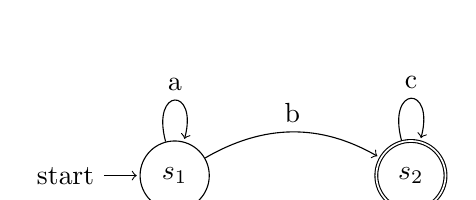
\begin{tikzpicture}[shorten >=1pt,node distance=2cm,on grid,auto]
      \node[state,initial] (q1) at (0,0) {$s_1$};
      \node[state,accepting] (q2) at (3,0) {$s_2$};
      \path[->] (q1) edge[loop above] node{a} (q1)
      (q2) edge[loop above] node{c} (q2)
      (q1) edge[bend left] node{b} (q2);
    \end{tikzpicture}
  \end{center}
  The resulting accepting formal language is:
  \[ \text{Set represntation: } L = \{a^nbc^n : n \in \mathbb{N}\}\]
  \[
    \text{Formal power series represntation: } L = a^*\cdot b\cdot c^* 
  = a^*bc^*
\]
\end{example}
% Define Formal languages (Sets and Power sereies) 
% and automatas (Tuple and Matrix)
\section{Formal Languages: Sets vs. Formal Power Series}
In this chapter, we will discuss the obvious differences and  similarities between both representations. First, we will give an intuition as to why one might use a series to represent a function definition.
Secondly, we will map the formal power series version into the set
version and the other way around, to get a better understanding of both.
Lastly, we will discuss why formal power series are more powerful
than just sets.\\
The intuition behind the notation of formal power series is quite simple.
The operation defined on the formal power series, which are maps, 
are really close to a series. In addition, formal power series and 
Normal series are quite similar, namely defined pointwise.\\
In the following are $L,V \in \fps{B}$ and $A,B$ series.
\[ 
  L + V = \sum_{w \in \Sigma^*} ((L,w) + (V,w))w \hspace{0.3cm}
  \leftrightarrow \hspace{0.3cm}
  A + B = \sum_{n \in \mathbb{N}} (a_n + b_n) x^n
\]
The multiplication defined on formal power series are again really close
to the Cauchy product of series.
In the following are $L,V \in \fps{B}$ and $A,B$ series.
\[
  L \cdot V = \sum_{\substack{u,v \in \Sigma^* \\ w=uv}} 
  ((L,u) \cdot (V,v))w
  \hspace{0.3cm} \leftrightarrow \hspace{0.3cm}
  A \cdot B = 
  \sum_{\substack{i,j \in \mathbb{N} \\ n = i + j}} (a_i \cdot b_j) x^n
\]
Consequently, it is quite handy to use a formal power series as a function definition, because the operations seem natural with series.
Despite the notation being quite confusing at first glance.\\
Next, we will show that both representations of a formal language are  equivalent, by mapping one to another.
To be sure that both representations are actually equivalent, we need to show there exists a bijective map between the formal power series and the set of words. 
This map needs to preserve the structure, which means the order of function application and operator application must be irrelevant.
Such maps are called isomorphisms, and the structures for that an isomorphism 
exist are called isomorphic to each other. Thus, we want to show that both representation are isomorphic.
\begin{proof}
  Let $\Sigma$ be an fixed alphabet, then we claim that:
  \[
    \mathbb{B}\langle \langle \Sigma^* \rangle \rangle
    \cong \mathcal{P}(\Sigma^*)\]
  In order to show those are isomorphic, we provide a map $\phi: 
  \mathbb{B}\langle \langle \Sigma^* \rangle \rangle \to \mathcal{P}(\Sigma^*)$ 
  and its inverse $\phi^{-1}: \mathcal{P}(\Sigma^*) \to \fps{B}$ and
  show that $\phi$ is bijective and preservers structure, formally:\\
  Let $L,V \in \fps{B}$, then for $\phi$ must hold:
  \begin{align}
    \phi(L + V) &= \phi(L) \cup \phi(V) \\
    \phi(L \cdot V) &= \phi(L) \cdot \phi(V)\\
    \phi(L^*) &= \phi(L)^*
  \end{align}
  We define $\phi$ and its inverse as follows:
  \[ 
    \phi(L) = \{ w \in \Sigma^* : (L,w) = 1\}
  \]
  \[
    \phi(L)^{-1} = h_{L}
  \]
  where
  \[ h_L: \Sigma^* \to \fps{B}\]
  \[
    h_L(w) = 
    \begin{cases}
      1, & \text{if} \hspace{0.2cm} w \in L \\
      0, & \text{otherwise}
    \end{cases}
  \]
  To prove that $\phi$ is bijective, it must hold
    \[ 
      \phi^{-1}(\phi(L)) = L
    \]
    and 
    \[
      \phi(\phi^{-1}(L)) = L.
    \]
    First we show $\phi^{-1}(\phi(L)) = L$\\
    Let $\ L \in \fps{B}$ abitrary but fixed, with 
    \[ L =\sum_{w \in \Sigma^*} (L,w)w. \]
    Then
    \begin{align*}
      \phi^{-1}(\phi(L)) = \phi^{-1}(\{ w \in \Sigma^* : (L,w) =1 \})
       &= 
       \begin{cases}
        1 & \text{if} \hspace{0.2cm} w \in \{ w \in \Sigma^* : (L,w) =1 \}\\
        0 & \text{otherwise}
       \end{cases}\\
       &= 
       \begin{cases}
        1 & \text{if} \hspace{0.2cm} (L,w) = 1\\
        0 & \text{otherwise}
       \end{cases}\\
       &= 
       \sum_{w \in \Sigma^*} (L,w)w = L.
    \end{align*}
    Next we need to show that $\phi(\phi^{-1}(L)) = L.$\\
    Let $\ L \in \mathcal{P}(\Sigma^*)$ abitrary but fixed, then
    \begin{align*}
      \phi(\phi^{-1}(L)) = \phi(h_L) = \{w \in \Sigma^* : (h_L,w) = 1 \}
      = \{ w \in \Sigma^* : h_L(w) = 1\} = \{ w \in \Sigma^* : w \in L\} = L.
    \end{align*}
    Consequently, $\phi$ is a one-to-one correspondence between formal power
    series and set of words.
    We are not done yet, we still need to prove that $\phi$ preserves
    structure, thus we need to show $(1), (2),$ and $(3)$. Starting with
    number one:
    \[ \text{\bf (1)} \hspace{0.3cm} \phi(L+V) = \phi(L) \cup \phi(V) \]
    In the following let $L,V \in \fps{B}$ arbitrary but fixed. Then
    \begin{align*}
      \phi(L+V) &= \{ w \in \Sigma^* : (L,w) + (V,w) = 1 \} \\
        &= \{ w \in \Sigma^* : (L,w) = 1 \lor (V,w) = 1 \} \\
        &= \{ w \in \Sigma^* : w \in \{ x \in \Sigma^* : (L,x) = 1 \}
        \lor w \in \{ x \in \Sigma^* :(V,x) = 1 \} \} \\
        &= \{ w \in \Sigma^* : w \in \phi(L) \lor w \in \phi(V) \} 
        = \phi(L) \cup \phi(V).
    \end{align*}
    Continuing with two:
    \[ 
      \text{\bf (2)} \hspace{0.3cm} 
      \phi(L\cdot V) = \phi(L) \cdot \phi(V) 
    \]
    In the following let $L,V \in \fps{B}$ arbitrary but fixed. Then
    \begin{align*}
      \phi(L\cdot V) &= \{ uv \in \Sigma^* : (L,u) \cdot (V,v) = 1\}\\
        &= \{ uv \in \Sigma^* : (L,u) = 1 \land (V,v) = 1\} \\
        &= \{ uv \in \Sigma^* : u \in \{ w \in \Sigma^* : (L,w) = 1\}
          \land v \in \{ w \in \Sigma^* : (V,w) = 1\}
        \} \\
        &= \{ uv \in \Sigma^* : u \in \phi(L)
          \land v \in \phi(V)
        \} = \phi(L) \cdot \phi(V).
    \end{align*}
    Last but not least, three:
    \[ 
      \text{\bf (3)} \hspace{0.3cm} 
      \phi(L^*) = \phi(L)^*
    \]
    In the following let $L \in \fps{B}$ arbitrary but fixed. Then
    \begin{align*}
      \phi(L^*) = \phi(\sum_{i\in \mathbb{N}_0} L^i) 
      \stackrel{\text{\bf (1)}}{=} \sum_{i\in \mathbb{N}_0} \phi(L^i)
      \stackrel{\text{\bf (2)}}{=} \sum_{i\in \mathbb{N}_0} \phi(L)^i
      = \phi(L)^*
    \end{align*}
    Thus $\phi$ is an isomorphism and our claim follows.
\end{proof}
\\\\
Now we have shown that both definitions are equivalent, but why should one use the less natural formal power series definition? The answer to this, as so often in mathematics, is {\bf abstraction}. Finite automata are accepting formal languages, thus we can say they generate a formal language.
 When abstracting from finite automata's to weighted automata's, which have a weight or cost between each transition, the generated object is not longer a language, but a map that assigns a weight or cost to each word. 
Generally, this weight or cost can be seen as a semi-ring (a ring that does not necessarily have an additive inverse), which are objects that behave like numbers. We will denote an arbitrary
semi-ring with $\mathbb{S}$. Those maps, that get accepted by a weighted
automata, have the signature $L: \Sigma^* \to \mathbb{S}$ and are 
indeed, a formal power series over $\mathbb{S}$, consequently $L \in \fps{S}$.
To summarize, finite automata generate formal power series over $\mathbb{B}$
and weighted automata generate formal power series over $\mathbb{S}$. So  formal power series are, in fact, an abstraction of formal languages.
\section{Kleene's theorem (Power series, Matrix Automata)}
In this chapter, we will examine, what kinds of languages get accepted by a finite automaton. In order to do that, we will prove that all languages that get accepted by an finite automaton are rational, and every rational language can be generated by a finite automaton (kleene's theorem).
A rational language is defined inductively.\\
\pagebreak
\begin{definition}
  Let $\Sigma$ be an fixed alphabet, then a rational language 
  is defined as follows:
  \begin{enumerate}
    \item A language $L = a \in \fps{B}$ with a single character 
      $a \in \Sigma$ is said to be rational.
    \item The empty word $\epsilon$ is rational.
    \item The sum of two rational Languages $L_1, L_2 \in \fps{B}$
      are again rational $L = L_1 + L_2$.
    \item The product of two rational Languages $L_1, L_2 \in \fps{B}$
      are again rational $L = L_1 \cdot L_2$.
    \item The kleene star of a rational language $L \in \fps{B}$ 
        is again rational $V = L^*$.
  \end{enumerate}
\end{definition}
So we start with just one character and then building with our operations step by step  a language. 
To show kleene's theorem, we have to prove two directions. 
First, we will prove that finite automata only accept rational  languages. 
Afterward, we will prove that every rational language is accepted by a finite automaton. 
In an effort to do that, we need to understand certain properties of the matrix encoding of finite automata.
Raising the power of two of a Matrix is defined by:\\
Let $A \in \fps{B}^{n\times n}$ be an arbitrary matrix, then
\[ 
  (A^2)_{ij} = \sum_{k=1}^{n} A_{ik}A_{kj}.
\]
As mentioned before, this matrix is a transition function of a finite
automata, where we can look up what character carries one state in another.
In $A_{ij}$ is the character that carries $i$ to $j$, thus multiplying
$A$ by itself gives us a new matrix with all words of length two, given as input, and $i$ is the starting node that would carry $i$ to $j$ in two steps. In the formula above, we see that we
are trying to go through all nodes $k \in \{1, 2, 3, \dots n\}$
to end up in $j$ and then uniting them together with addition.\\
Generally, we can have a matrix $A \in \fps{B}^{n \times n}$
risen to the power of $n \in \mathbb{N}$:
\[
  (A^n)_{ij} = \sum_{k_1=1}^{n}
    \sum_{k_2=1}^{n}\dots \sum_{k_{n-1}=1}^n 
    a_{ik_1}a_{k_1k_2}a_{k_2k_3}\dots a_{k_{n-1}j} \\
\]
This is not beautiful at all, but the idea stays exactly the same: now we have in $(A^n)_{ij}$ all words that carry $i$ to $j$ in n steps, brute forcing through all possible paths. Now to get all possible paths of arbitrary length, we just add them all together:
\[
  E_n + A + A^2 \dots = \sum_{i \in \mathbb{N}} A^i = A^*
\]
Yielding, that in $(A^*)_{ij}$ are all possible words, carrying the automata from $i$ to $j$. If $i$ is the starting node and $j$ the accepting node, the accepting language of the automata is just
$(A^*)_{ij}$. That means, $A^*$ stores all accepting languages of  an automaton, with transition matrix $A$.
With those important properties, we can now move on to the first prove.
\\ 
\pagebreak
\\
\begin{proof}
  \begin{center}
    {\bf claim: All finite automata only accept rational languages.}
  \end{center}
  Let $A \in \fps{B}^{n \times n}$ be a transition function of an
  arbitrary finite automata. $A$ is rational because the transition
  function consists only out of characters. Since $A^*$ stores every accepting
  language of that finite automata, for every possible initial
  state and accepting state, we just need to prove that all entries
  in $A^*$ are rational languages.
  We will prove this statement via induction over the number of 
  states, namely the dimension of the square matrix $n \in \mathbb{N}$.\\
  {\bf Base case: $n=1$}\\
  Thus
  \[
    A \in \fps{B}^{1 \times 1} = \fps{B}.
  \]
We know that $A \in \fps{B}$ is rational, but that also means  that $A^*$ is per definition rational, which finishes the base case.\\
{\bf Induction step: $n \to n+1$}\\
We can assume the claim holds for $n \in \mathbb{N}$ and need to prove it
also holds for $n+1$. Thus, we can assume that a transition matrix with
dimension $n \times n$ has only rational entries. \\
Let $A \in \fps{B}^{(n+1) \times (n+1)}$ be a transition function of an
arbitrary finite automata. 
Our goal is to reduce the square matrix $A$ by one dimension.
In order to do that, we divide the matrix into four blocks:
\[
  A = 
  \begin{pmatrix}
    A(1,1) & A(1,2) \\
    A(2,1) & A(2,2)
  \end{pmatrix}
\]
where 
\[ 
  \textcolor{brown}{ A(1,1) }\in \fps{B}^{1 \times 1},
  \textcolor{orange}{ A(2,1)} \in \fps{B}^{n \times 1}, 
  \textcolor{blue}{A(1,2)} \in \fps{B}^{1 \times n},
  \textcolor{red}{A(2,2)} \in \fps{B}^{(n-1) \times (n-1)}
\]
visually:
\begin{center}
  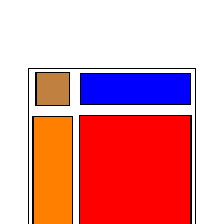
\begin{tikzpicture}[square/.style={regular polygon,regular polygon sides=4}]
      \node at (0,0) [square,draw,minimum width=3cm] (m) {};
      \node at (0.3,0.8) [rectangle,draw,minimum height=0.4cm,minimum width=1.4cm,fill=blue] (m21) {};
      \node at (-0.75,-0.25) [rectangle,draw,minimum height=1.4cm,minimum width=0.5cm,fill=orange] (m12) {};
      \node at (0.3,-0.25) [square,draw,minimum width=2cm,fill=red] (m) {};
      \node at (-0.75,0.8) [square,draw,minimum width=0.6cm,fill=brown] (m) {};
  \end{tikzpicture}
\end{center}
We can interpret our block matrix as a transition matrix with four entries,
thus having two states. Our new two states consist of the original states in the following way:
\[
  \mathbf{1} = \{1\} \text{ and } \mathbf{2} = \{2,3,4, \dots n + 1\}
\]
\\
\pagebreak
\\
We can visulize the resulting automata:
\begin{center}
  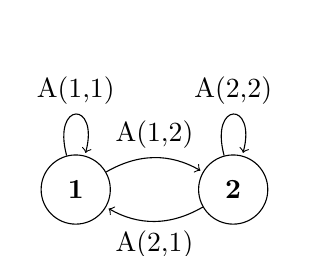
\begin{tikzpicture}[shorten >=1pt,node distance=2cm,on grid,auto] 
    \node[state] (q_0)   {$\mathbf{1}$}; 
    \node[state](q_1) [right=of q_0] {$\mathbf{2}$};
      \path[->] 
      (q_0) edge[bend left, above]  node {A(1,2)} (q_1)
            edge [loop above] node {A(1,1)} ()
      (q_1) edge[bend left, below]  node {A(2,1)} (q_0)
            edge [loop above] node {A(2,2)} ();
  \end{tikzpicture}
\end{center}
Now, instead of calculating $A^*$ with algebra, we can also just look
at the automata and ponder what all possible paths are for $1 \to 1$,
$1 \to 2$, $2 \to 1$, and $2 \to 2$. Note that the automaton is symmetrical, consequently we just need to find paths for $1 \to 1$ and $1 \to 2$.
Starting with $1 \to 1$, we want to find all possible paths from state
one to one with an arbitrary length. Starting at state one, we can either
directly loop back to one, or we transition to two, then loop in two 
arbitrary amount of times and then transition back to one. This whole
process can also be repeated an arbitrary amount of times, yielding the
following formula:
\[
  A(1,1)^* = (A(1,1) + A(1,2)A(2,2)^*A(2,1))^*
\]
Now, because of symmetry:
\[
  A(2,2)^* = (A(2,2) + A(2,1)A(1,1)^*A(1,2))^*
\]
For $1 \to 2$, we can loop in one and then transition to two, in two 
We can either loop there for an arbitrary amount of time or transition to one loop in one an arbitrary amount of times and then go back to
two. This process can also be repeated an arbitrary amount of times.
\[
  A(1,2)^* = A(1,1)^*A(1,2)(A(2,2)^* + A(2,1)A(1,1)^*A(1,2))^*
\]
Again because of symmetry:
\[
  A(2,1)^* = A(2,2)^*A(2,1)(A(1,1)^* + A(1,2)A(2,2)^*A(2,1))^*
\]
The transition matrix $A^*$ has only rational entries, if all blocks
matrices only have rational entries. The block matrices consist of, 
just entries of $A$ that are rational, namely $A(1,1)$, $A(2,2)$, $A(1,2)$
and $A(2,1)$. As well as square matrices, which have
a lower dimension than $n+1$, thus the kleene stars of those are also 
rational because of the induction assumption, namely 
$A(2,2)^*$, $A(1,1)^*$, $(A(1,1)^* + A(1,2)A(2,2)^*A(2,1))^*$, 
$(A(2,2)^* + A(2,1)A(1,1)^*A(1,2))^*$, $(A(2,2) + A(2,1)A(1,1)^*A(1,2))^*$
and $(A(1,1) + A(1,2)A(2,2)^*A(2,1))^*$. Thus, $A^*$ has only rational
entries, which finishes the proof.
\end{proof}\\
\pagebreak
\\
Now, we have to prove the other direction:
\begin{proof}
  \begin{center}
    {\bf claim: Every rational language can be generated 
    by an finite automata.}
  \end{center}
    Previously in this chapter, we defined rational language inductively,  naturally we want to prove the claim with structural induction. That  means we need to construct an automata generating...
  \begin{enumerate}
    \item ... a language with one letter.
    \item ... the product of two languages.
    \item ... the sum of two languages.
    \item ... the kleene star of one language.
  \end{enumerate}
  In the following, all constructed automata will have the first
  state as initial state and all states as accepting state.
  Thus, the sum of the first row of the transition
  matrix $A^*$ will be the accepted language.
  We begin to prove that {\bf (1)} there are an automaton accepting a
  single letter.\\
  Let $\Sigma$ be an arbitrary but fixed alphabet and 
  $\alpha \in \Sigma$ a letter, then:
  \[
    A = 
    \begin{pmatrix}
      \epsilon & \alpha\\
      0        & \epsilon
    \end{pmatrix}
  \]
    Looking at the automata and ponder again, like in the previous proof, we see that $A = A^*$.
  \begin{center}
    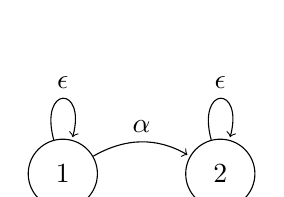
\begin{tikzpicture}[shorten >=1pt,node distance=2cm,on grid,auto] 
      \node[state] (q_0)   {$1$}; 
      \node[state](q_1) [right=of q_0] {$2$};
        \path[->] 
        (q_0) edge[bend left, above]  node {$\alpha$} (q_1)
              edge [loop above] node {$\epsilon$} ()
        (q_1) edge [loop above] node {$\epsilon$} ();
    \end{tikzpicture}
  \end{center}
  With our convention,
  we get the accepted language $L = \epsilon + \alpha$, thus $\alpha \in L$.\\
  Next, we will look at the sum of two rational language {\bf (2)}. Let $A,B \in \fps{B}^{n \times n}$ transition matrices of rational languages, then
  \[
    B = 
    \begin{pmatrix}
      \epsilon & A_1 & B_1 \\
      0        & A   & 0 \\
      0        & 0   & B
    \end{pmatrix}
  \]
  where 
  \[
    A_1 = (a_{11}, a_{12}, a_{13}, \dots a_{1n})
    \hspace{0.2cm} \text{and} \hspace{0.2cm}
    B_1 = (b_{11}, b_{12}, b_{13}, \dots b_{1n}).
  \]
  \\
  \pagebreak
  \\
  Depicting the automata: 
  \begin{center}
    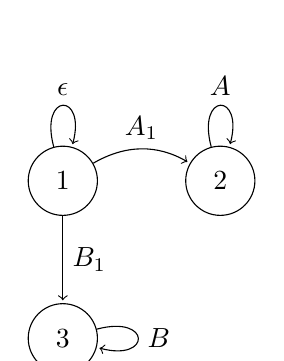
\begin{tikzpicture}[shorten >=1pt,node distance=2cm,on grid,auto] 
      \node[state] (q_0)   {$1$}; 
      \node[state](q_1) [right=of q_0] {$2$};
      \node[state](q_2) [below=of q_0] {$3$};
        \path[->] 
        (q_0) edge[bend left, above]  node {$A_1$} (q_1)
              edge [loop above] node {$\epsilon$} ()
              edge [] node {$B_1$} (q_2)
        (q_1) edge [loop above] node {$A$} ()
        (q_2) edge [loop right] node {$B$}();

    \end{tikzpicture}
  \end{center}
  With the same reasoning as above we get:
  \[
    B^* = 
    \begin{pmatrix}
      \epsilon & A_1A^* & B_1B^*\\
      0        & A^*    & 0 \\
      0        & 0      & B^*
    \end{pmatrix}
  \]
  where 
  \[
    A_1A^* = (\sum_{k=1}^{n}a_{1k}a^*_{k1}, \sum_{k=1}^{n}a_{1k}a^*_{k2},
        \sum_{k=1}^{n}a_{1k}a^*_{k3}, \dots \sum_{k=1}^{n}a_{1k}a^*_{kn})
        = A\hat{}_1
  \]
  and 
  \[
    B_1B^* = (\sum_{k=1}^{n}b_{1k}b^*_{k1}, \sum_{k=1}^{n}b_{1k}b^*_{k2},
        \sum_{k=1}^{n}b_{1k}b^*_{k3}, \dots \sum_{k=1}^{n}b_{1k}b^*_{kn})
        = B{\mathchar"5E}_1.
  \]
  Yielding the first row sum $L = \epsilon + A\hat{}_1 + B{\mathchar"5E}_1$,
  which is exactly the sum of the accepted language of $A$ and $B$.\\
  Next, we will look at the product of two rational language {\bf (3)}.
  Let $p,q\in \mathbb{N}$, $A \in \fps{B}^{p \times p}$ and $B \in \fps{B}^{q \times q}$ transition matrices of rational
  languages, then
  \[
    C = 
    \begin{pmatrix}
      A & PQ \\
      0 & B
    \end{pmatrix}
  \]
  where
  \[ P \in \fps{B}^{p \times q}, \hspace{0.2cm}Q \in \fps{B}^{q \times p}\]
  \[
    P_{ij} = 
    \begin{cases}
      \epsilon & \text{if } \hspace{0.2cm} j = 1\\
      0        & \text{otherwise}
    \end{cases}
    , \hspace{1cm}
    Q_{ij} = 
    \begin{cases}
      \epsilon & \text{if } \hspace{0.2cm} j = 1 \land i = 1\\
      0        & \text{otherwise}
    \end{cases}
  \]
  \\
  \pagebreak
  \\
  Using the formula of the last proof we get:
  \[
    C^* = 
    \begin{pmatrix}
      A^* & A^*PQB^* \\
      0 & B^*
    \end{pmatrix}
  \]
  where
  \[
    (A^*P)_{ij} = 
    \begin{cases}
      \sum_{k=1}^{p} a^*_{1k}p_{k1} =  \sum_{k=1}^{p} a^*_{1k} 
        & \text{if } \hspace{0.2cm} i = 1 \land j = 1\\
      \sum_{k=1}^{p} a^*_{ik}p_{k1} =  \sum_{k=1}^{p} a^*_{ik} 
        & \text{if } \hspace{0.2cm} i > 1\land j = 1\\
      0 & \text{otherwise}
    \end{cases}
  \]
  and 
  \[
    (QB^*)_{ij} = 
    \begin{cases}
      \sum_{k=1}^{p} q_{1k}b^*_{kj} = b^*_{1j}
        & \text{if } \hspace{0.2cm} i = 1\\
      0  & \text{otherwise}
    \end{cases}
  \]
  We are only interested in the first row:
  \[
    (A^*PQB^*)_{1j} = \sum_{k=1}^{q} (A^*P)_{1k}(QB^*)_{kj} 
      = (A^*P)_{11}(QB^*)_{1j}
      = (\sum_{k=1}^{p} a^*_{1k})b^*_{1j}
  \]
  Summing the whole row of $C^*$ together to get the accepted language: 

  \[
    L = (\sum_{k=1}^{p} a^*_{1k}) + \sum_{j=1}^q (\sum_{k=1}^{p} a^*_{1k})b^*_{1j}
      = (\sum_{k=1}^{p} a^*_{1k}) + (\sum_{k=1}^{p} a^*_{1k}) (\sum_{j=1}^q b^*_{1j})
      = (\sum_{k=1}^{p} (A^*_1)_k) + (\sum_{k=1}^{p} (A^*_1)_k) (\sum_{j=1}^q (B^*_1)_j)
  \]
  We get the accepted language of $A$ times the accepted language of $B$.\\
  Last but not least, we need to prove that there exists an automaton which
  gives us the kleene star of a rational language. Let 
  $p,q\in \mathbb{N}$ and $A \in \fps{B}^{p \times p}$
  a transition matrix of a rational language 
  and  $P \in \fps{B}^{p \times q}$, $Q \in \fps{B}^{q \times p}$
  like above, then
  \[
    D := 
    \begin{pmatrix}
      E_p &  E_p\\
      0        & A + PQ
    \end{pmatrix}
  \]
  Again, with the formula of the former proof, we get:
  \[
    D^* = 
    \begin{pmatrix}
      E_p &  (A + PQ)^*\\
      0   &  (A + PQ)^*
    \end{pmatrix}
  \]
  The element in the upper right corner can be rewritten:
  \[
    (A+PQ)^* = A^*(PQA^*)^*
  \]
  The sum of the elements in the first row yields $L^*$.
\end{proof}
\section{Conclusion}
The former prove can be modified to also hold for formal power series in
a semi-ring $\fps{S}$ (ref. [\cite{Algebra}]). 
This theorem is called kleene-schützberg theorem (ref. [\cite{Algebra}]) and
it makes a connection between formal power series and weighted automata. 
In summary, formal power series are really powerful, but also quite
unintuitive at first. For futher reading my recommendation is the master thesis
of Laura Wirth (ref. [\cite{master}]).
\pagebreak
\addcontentsline{toc}{section}{Bibliography}
\pagestyle{fancy}
\bibliographystyle{language-dt} 
\bibliography{bibliography} 
%\nocite{*}
\end{document}
